\clearpage 

\section*{Abberviations}

\begin{tabular}{ll}
	LMI & linear matrix inequality 
	\\ LP & linear program or linear programming 
	\\ NLP & non-linear program or non-linear programming 
	\\ POP & polynomial optimization program or polynomial optimization
	\\ PSD & (symmetric) positive semidefinite
	\\ SDP & (linear) semidefinite optimization program or semidefinite programming
	\\ SOS & sum of squares
\end{tabular}

\clearpage 

\section*{About these notes} 

In July 2017, Prof.~Sebastian Sager and I held a course aiming at presenting some of the trends in modern optimization. This course is one of the teaching activities of the Research Training Network Mathematical Aspects of Complexity Reduction, supported by the German Research Foundation. Sebastian presented various aspects of linear, non-linear, mixed-integer and global optimization and also addressed optimization in infinite-dimensional spaces (in systems and control theory). 

In my part of the course, I explained the reduction of polynomial optimization problems to semidefinite optimization via the sum-of-squares approach, and explained how the interior point methods can be used to solve semidefinite problems based on the duality of semidefinite programming. This manuscript presents the notes, on which my part of the course was based.

Currently, there are several regular sources, from which you can learn about the topic: a long expository article of Monique Laurent~\cite{laurent2009sumsofsquares}, the book of Jean B.~Lasserre~\cite{lasserre2015anintroduction}, which is the standard reference book in polynomial optimization and the book of Murray Marshall~\cite{marshall2008positivepolynomials} that contains the necessary theoretical background from real algebra and ends with a short discussion of polynomial optimization.  There are basic dual approaches to reduce polynomial problems to semidefinite programming: one can use sum-of-squares relaxations and truncated-moment relaxations. In my notes, I discuss truncated-moment relaxations very briefly and towards the end of the notes. The line of thought is as follows: 
\begin{enumerate}
	\item To obtain lower bounds we need algebraic certificates for positivity; Sums of squares of polynomials turn out to be a very nice tractable certificate that can be expressed in terms of semidefinite optimization. Unfortunately, one cannot use sums of squares of polynomials to always certify positivity.
	\item One can always use sums of squares of rational functions, which shows that positivity is intrinsically related to sums of squares.
	\item On compact semialgebraic sets, positivity \emph{can} be expressed through sums of squares of polynomials. 
	\item For solving semidefinite problems, one needs to understand duality of semidefinite programming, which is a special case of conic duality. 
	\item Semidefinite programs can be solved using interior point methods. 
\end{enumerate}

Each of the above points corresponds to a chapter of these notes. Discussing point~3 I rely on my short exposition article \cite{averkov2013constructive} on elementary approaches to denominator-free positivstellensätze, which collects various pieces of information that were spread all over the literature. 

I made no attempt to give an extensive exposition of the background literature (though I plan to extend the literature list in the future).

A second iteration of the compact course based on these notes was held by Maximilian Merkert in 2020, whom I would like to thank for implementing some corrections compared to the initial version.

If you happen to spot any issues (inconsistencies etc.), please let me know. 

\clearpage 

\section{Introduction}



\subsection{Global non-linear optimization} 

\begin{itemize}
	%
	\item Convex and linear optimization problems are computationally tractable. This is confirmed in theory and practice! One very special thing about convex optimization is that there is no difference between local and global optimality. So, for checking global optimality, local information is enough.
	%
	\item In applications, one frequently needs to solve non-linear problems. When one says \emph{non-linear} one usually means \emph{non-convex problems}, because in optimization the crucial difference is not between linear and non-linear but between convex and non-convex.
	%
	\item Originally, one is usually interested in \emph{global non-linear optimization}. Of course, when the underlying global optimization problem is hard, one can try to find a locally optimal solution rather than solving the problem globally. However, if there are lots of local solutions of all possible qualities, why should a `random' local solution be good?  See figure: if you pick any locally optimal solution, you will get as good as any value of the objective function. So, why is a locally optimal solution any better than just any solution?
	\begin{center}
		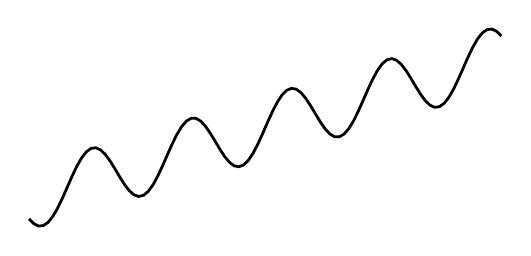
\begin{tikzpicture}
			\draw[line width=1pt,domain=-3:3,samples=100] plot ({\x}, {0.3*\x+0.4*sin(5*deg(\x))}); 
		\end{tikzpicture}
	\end{center}
%	\begin{center}
%		\begin{tikzpicture}
%		\begin{axis}[domain=0:3,legend pos=outer north east,,samples=100]
%		\addplot {0.3*x+0.2*sin(10*deg(x))}; 
%		%\legend{$x+ 6 \sin(x)$}
%		\end{axis}
%		\end{tikzpicture}
%	\end{center}
	%
	\item So, if we are really interested in solving an original problem, we usually have to deal with global non-linear programming (NLP).
	%
	\item \emph{General} global NLP is extremely hard. It's a \emph{huge} class of problems. Depending on how you define it, not algorithmically solvable. Consider the feasibility problem 
	\begin{align*}
		\sin(\pi x_1) = \ldots = \sin(\pi x_n) & = 0 & & \text{(Integrality constraints $x_1,\ldots,x_n \in \Z$)}
		\\ p(x_1,\ldots,x_n) & = 0 & & \text{(Polynomial equality)}
	\end{align*}
	It is not algorithmically solvable (see Matyasievich's answer to Hilbert's 10th problem). If you do not like the feasibility formulation you can reword the problem equivalently as an optimization problem. Just ask whether the optimal value of the minimization problem
	\[
		\inf \setcond{p(x_1,\ldots,x_n)^2 + \sum_{i=1}^n \sin(\pi x_i)^2}{x=(x_1,\ldots,x_n) \in \R^n} 
	\]
	is $0$ and if this value is attained for some $x \in \R^n$.
	
	%
	\item Take a look at the \blue{following chain of complexity classes}
	\[
		\complP \subseteq \complNP \subseteq \complPSPACE \subseteq \complEXP \subseteq \complDECIDABLE
	\]
	It is conjectured that all inclusions are strict and the inclusion $\complP \subseteq \complEXP$ is known to be strict. As we have seen, global NLP is not decidable and so it is easy to imagine that subclasses of global NLP are spread all over this chain. So, \blue{they cover} lots of extremely difficult problems, including the $\complNP$-complete problems, which researchers have already been working \blue{on} for decades. 
	
	Complexity theory tells us that there is no way of finding a \emph{universal} efficient approach to very hard problems. Still, we can and will develop some quite general theory which can help us to do appropriate algorithmic choices for our concrete problems we want to solve. 
	%
	\item Currently, the global NLP community seems to be split into two sub-communi\-ties:
    \begin{itemize}
	 \item One can use
  	 \begin{itemize}
		\item branching,
		\item introducing intermediate variables to keep track of the intermediate results in the expression digraphs of the underlying functions, or
		\item basic outer convexification (McCormick, $\alpha$-relaxations  et al.)
	\end{itemize}
	Such techniques are available in solvers like Baron. 

    \item Alternatively, one can use sums-of-squares which has also been implemented.
    \end{itemize}
\end{itemize}
	
\subsection{Polynomial optimization}

I what follows, I am going to use POP to abbreviate either \emph{polynomial optimization} or a \emph{polynomial optimization problem}. 

POP is the class of problems of dealing with optimization of
\begin{itemize}
	\item a polynomial objective function 
	\item in the presence of finitely many real-valued decision variables and 
	\item under finitely many polynomial equality/inequality constraints
\end{itemize}

Direct usage of equality constraints can be avoided, as we can replace $p(x)=0$ by $p(x) \ge 0$ and \blue{$-p(x) \ge 0$}. When we talk about inequality constraints, we mean the non-strict inequalities by default, but it can easily be seen that strict inequalities can be easily modelled via non-strict ones in lifting in the context of POP. Indeed $p(x) >0$ can be expressed as $p(x) y = 1$ and $y \ge 0$ using an additional variable $y$. 

We'll see how POPs can be converted to so-called semidefinite problems (SDPs). Some more specific situations can also be converted to linear problems (LPs). For LPs and SDPs various efficient solution methods can be employed. 

General POP involves a lot of kinds of problems as special cases, including the following $\complNP$-hard) problems:
\begin{itemize}
	\item Binary integer linear programming (so there is a connection to \emph{combinatorial optimization})
	\item Inequality constrained quadratic programming (and so there is a connection to classical numerical \emph{nonlinear optimization} dealing with iterative methods based on first and second derivatives and Taylor expansions). 
\end{itemize}

Since on a compact set, every continuous function can be approximated by a polynomial (Stone-Weierstrass theorem) with any given accuracy, in some sense, POP is dense in NLP. Apart from that, polynomials provide a very natural `modeling language', because arithmetics over reals (multiplication and addition) is one of the basic things a computer can do.  

There exist results showing that the decision version of polynomial optimization is in $\complEXP$ (see \cite{MR3212780}), so polynomial optimization (in its decision form) is somewhere between $\complNP$-hard and $\complEXP$ (but I do not know its precise complexity). 

%In my part of the lectures I would like to present algebraic approaches to \emph{global} nonlinear programming. We consider the family POP of polynomial optimization problems which is a very interesting subset of NLP. One can define POP as problems of optimizing a polynomial function on $\R^n$ subject to a finite system of non-strict polynomial inequalities (equalities can be easily modeled through inequalities). In some sense, POP is almost equal to NLP (kind of dense subset). Sebastian Sager has already presented the main approaches of the `non-linear optimization community' to NLP. 

%From the mathematical viewpoint, POP is interesting because of its relations to algebra,a and the hope is that algebraic theory may help for POP. Many concrete examples of NLP problems are actually POP problems. 

%In last decades, beautiful solutions techniques for POP have been developed which based on reduction of POP to convex problems through the so-called semidefinite optimization. POPs can be reduced to a hierarchy of large-size semidefinite problems (SDPs). This reduction is based on a certain duality theory for POP (Positivstellensätze). One can solve SDPs using interior-point methods for conic programming. Note that SDP is a far-reaching generalization of LP (One has LP $\subseteq$ SOP $\subseteq$ SDP, where SOP is a second-order cone programming, and all the paradigms are interesting in their own right). There exist interior-point methods tailored to conic problems, most notably to SDPs.

\subsection{Prerequisites}

The more you know about the following topics, the easier it would be for you to follow the discussion. 

\begin{itemize}
	\item[] \emph{Linear algebra}. Vector spaces, Euclidean spaces, linear maps. 
	\item[] \emph{Convexity}. Convex sets and cones, polyhedra, separations theorems, faces and extreme points. In the standard mathematics curriculum, convexity is usually integrated into introductory optimization courses.
	\item[] \emph{Linear optimization}. Duality, understanding the geometry of the simplex method. 
	\item[] \emph{Analysis}. Basic knowledge. 
	\item[] \emph{Algebra}. A bit of experience with groups, rings (and ideals), and fields. 
\end{itemize}

\subsection{Notation} 

\begin{tabular}{lll}
Set relations:	& & 
\\		& $\subseteq$ & regular inclusion 
\\ 		& $\varsubsetneq$ & proper inclusion
\\ Sets of numbers: & &
\\ & $\N$  & positive integers (called natural numbers here)
\\ & $\Z_+$ & non-negative integers
\\ & $\Q$ & rational numbers
\\ & $\R$ & real numbers
\\ & $\compl$ & complex numbers
\\ & $\R_+$ & non-negative reals 
\\ & $\R_{\ge 0}$ & non-negative reals (another notation)
\\ & $\R_{>0}$ & positive reals
\\ & $[m]$ & natural numbers not greater than $m \in \Z_+$
\\ Operations for sets: & & 
\\ & $\intr$ & interior
\\ &  $\conv$ & convex hull
\\ &  $\cone$ & \emph{convex} conic hull
\\ & $\lin$ & linear hull
\\ & $\aff$ & affine hull
\end{tabular} 

We use $0$ to denote the zero element; it can be zero value, zero vector or a zero matrix, depending on the context. 

Throughout, $n \in \N$ is the dimension of the ambient space, which is usually $\R^n$. The elements of $\R^n$ are viewed as columns, but we tend to omit transposition to simplify the expressions. For example, we write $(1,2,3) \in \R^3$ rather than $(1,2,3)^\top \in \R^3$. If $I$ is a set, then $\R^I$ is the set of all functions from $I$ to $\R$ and it can also be viewed (and written) as a vector indexed by elements of $I$. So, we can write for example $x=(x_i)_{i \in I} \in \R^I$. With this point of view, $\R^n$ is nothing but a special case of $\R^I$ with $I=[n]$. Please note that we do not insist $x_i$ to be the default notation for the $i$-component, because in cases we do not work with components of vectors, we prefer to use lower indexing for vectors. 

For $x= (x_i)_{i \in [n]}$ and $y = (y_i)_{i \in [n]}$, we introduce the standard scalar product $\sprod{x}{y} = \sum_{i=1}^n x_i y_i$ of $x$ and $y$ and the respective Euclidean norm $\|x\| := \sqrt{\sprod{x}{x}}$ of $x$. We also use the notation $\sprod{\dotvar}{\dotvar}$ and $\|\dotvar\|$ to denote the scalar product and the respective norm of other Euclidean spaces appearing in our discussion. The scalar product gives rise to the orthogonality relation and we use the notation $X^\perp$ to denote the orthogonal complement of $X$ (which is the set of all vectors orthogonal to every vector from $X$). 

By $I_n$ we denote the identity matrix of size $n$, and if the size is clear from the context we omit the subscript $n$. If $A$ is a matrix, then $A^\top$ denotes the transpose of~$A$. When we say that a matrix $A$ is PSD we always mean symmetric PSD.



Asymptotic notation for $f, g: X \to \R$, for $x \to x^\ast$:

\begin{center}
\begin{tabular}{l@{\hskip 5em}l}
	$f=O(g)$ & $\limsup_{x \to x^\ast} \frac{|f(x)|}{|g(x)|} < +\infty$ 
	\\ $f=\Omega(g)$ & $\liminf_{x \to x^\ast} \frac{|f(x)|}{|g(x)|} < +\infty$ 
	\\ $f = \Theta(g)$ & $f= O(g)$ and $f = \Omega(g)$
	\\ $f = o(g)$ & $\lim_{x \to x^\ast} \frac{|f(x)|}{|g(x)|} = 0$. 
\end{tabular}
\end{center}


By $\R[X_1,\ldots,X_n]$ we denote the set of polynomials in variables $X_1,\ldots,X_n$ with coefficients in $\R$. Instead of $\R$ one can use other sets, so one can consider other sets of polynomials, but we'll mostly work with $\R[X_1,\ldots,X_n]$. A warning for those, who don't have much experience with algebra: polynomials and functions are not quite the same thing. Rather, polynomials are formal expressions, and their variables $X_1,\ldots,X_n$ are just formal symbols (also called \emph{indeterminates}). So, a symbolic variable $X$ in the ring $\R[X]$ of univariate polynomials with real coefficients is not equal to any element of $\R$, because $X$ is just another element of $\R[X]$ (as any element of $\R$). To illustrate this, consider the following code in sage which introduces a symbol variable and compares it to the number $3$: 

\begin{verbatim}
x = var('x')
if x!=3:
   print "Not equal"
else:
   print "Equal"
\end{verbatim}

You can try this code at \url{http://sagecell.sagemath.org/}. Another way to explain this is by means of coefficients. The element $3$ of $\R[X]$ is a degree one polynomial, that is $3 = 3 + 0 X + 0 X^2 + \ldots $, and its coefficients are $3, 0, 0, \ldots$. On the other hand $X$ is another polynomial $X = 0  + 1 X + 0 X^2 + \cdots$ and its coefficients are $0, 1,0 , 0, \ldots$. Comparison of polynomials is defined through comparision of coefficients and so $3$ and $X$ are not equal, because their respective coefficients are not all equal. 

$\R(X_1,\ldots,X_n)$ denotes the set of rational functions in $X_1,\ldots,X_n$ with coefficients in $\R$. Even though rational functions are called functions, they are not functions but formal quotients $f/g$ with $f, g \in \R[X_1,\ldots,X_n]$ and $g \ne 0$. By definition, two such functions $f_1/ g_1$ and $f_2/g_2$ are equal if the polynomial equality $f_1 g_2 = f_2 g_1$ holds. 

For various kinds of structures \blue{$X$ and $Y$,} we use notations like $X + Y = \setcond{ x + y}{x \in X, y \in Y}$, $X - Y = \setcond{x - y}{x \in X, y \in Y}$, $a X = \setcond{ a x }{x \in X}$ etc. This allows us to express things in a concise form. For example, if $R$ is a ring, then an ideal $I$ of $R$ can be defined as an additive subgroup of $R$ satisfying $R I \subseteq I$, where we use the notation $X Y = \setcond{x y }{x \in  X, y \in Y}$. 


\subsection{Numbering}

Theorems, Lemmas, Propositions, Remarks, Exercises and Examples are all numbered based on a common counter. In my opinion, this simplifies searching. 

\subsection{Software}

The following software will or may be useful:

\begin{center}
\begin{tabular}{lp{9.7cm}c}
	\textbf{Name} & \textbf{Description} & \textbf{Used}
	\\ \hline MATLAB & proprietary numerical computing environment & yes
	\\ GNU Octave & free alternative for MATLAB & no
	\\ \hline AMPL & modelling language for optimization problems & yes
	\\ \hline SeDuMi & MATLAB package for solving semidefinite problems & yes
	\\ \hline SOSTOOLS & sums-of-squares based optimization toolbox for MATLAB & yes
	\\ GloptyPoly & sums-of-squares and moment-relaxation based optimization toolbox for MATLAB & no
	\\ \hline BARON software &  global solver for non-convex problems & yes
\end{tabular}
\end{center}

One could have listed more software.

